%!TEX root = ../main.tex
% Chapter 10 — Eigenvalues and Eigenvectors

\chapter{Numerical Computation of Eigenvalues and Eigenvectors}
\label{ch:eigenvalues}


\section{Introduction}

The eigenvalue problem---finding $\lambda$ and $\mathbf{v} \neq \mathbf{0}$ such that $\mathbf{A}\mathbf{v} = \lambda\mathbf{v}$---arises throughout science and engineering: vibration analysis, stability of dynamical systems, principal component analysis, Google's PageRank, and quantum mechanics, among many others. Since the eigenvalues are roots of the characteristic polynomial $\det(\mathbf{A} - \lambda\mathbf{I}) = 0$, and there is no closed-form formula for roots of polynomials of degree $\geq 5$ (Abel--Ruffini theorem), all general eigenvalue algorithms are necessarily \emph{iterative}.

%==============================================================================
\section{Spectral Properties}
%==============================================================================

\begin{definition}[Spectrum]
\label{def:spectrum}
\index{spectrum}
The \textbf{spectrum} of $\mathbf{A} \in \R^{n \times n}$ (or $\C^{n \times n}$) is the set of its eigenvalues:
\[
    \sigma(\mathbf{A}) = \{\lambda \in \C : \det(\mathbf{A} - \lambda\mathbf{I}) = 0\}.
\]
The \textbf{spectral radius} is $\rho(\mathbf{A}) = \max_{\lambda \in \sigma(\mathbf{A})} |\lambda|$.
\end{definition}

\begin{proposition}[Basic spectral properties]
\label{prop:spectral}
Let $\mathbf{A} \in \C^{n \times n}$ with eigenvalues $\lambda_1, \ldots, \lambda_n$ (counted with multiplicity).
\begin{enumerate}
    \item $\displaystyle\sum_{i=1}^n \lambda_i = \operatorname{tr}(\mathbf{A})$, \qquad $\displaystyle\prod_{i=1}^n \lambda_i = \det(\mathbf{A})$.
    \item If $\mathbf{A}$ is real and $\lambda \in \sigma(\mathbf{A})$, then $\bar{\lambda} \in \sigma(\mathbf{A})$.
    \item If $\mathbf{A}$ is symmetric (Hermitian), all eigenvalues are real.
    \item If $\mathbf{A}$ is symmetric positive definite, all eigenvalues are positive.
    \item $\sigma(\mathbf{A}^{-1}) = \{1/\lambda : \lambda \in \sigma(\mathbf{A})\}$ when $\mathbf{A}$ is invertible.
    \item $\sigma(\mathbf{A} - \sigma\mathbf{I}) = \{\lambda - \sigma : \lambda \in \sigma(\mathbf{A})\}$ (spectral shift).
\end{enumerate}
\end{proposition}

%==============================================================================
\section{Gerschgorin's Theorem}
%==============================================================================

\begin{theorem}[Gerschgorin circle theorem]
\label{thm:gerschgorin}
\index{Gerschgorin theorem}
Every eigenvalue of $\mathbf{A} \in \C^{n \times n}$ lies in at least one of the \textbf{Gerschgorin discs}:
\[
    D_i = \left\{ z \in \C : |z - a_{ii}| \leq R_i \right\}, \qquad R_i = \sum_{\substack{j=1 \\ j \neq i}}^{n} |a_{ij}|.
\]
That is, $\sigma(\mathbf{A}) \subset \bigcup_{i=1}^{n} D_i$.

Moreover, if a union of $k$ discs is disjoint from the remaining $n-k$ discs, it contains exactly $k$ eigenvalues (counted with multiplicity).
\end{theorem}

\begin{proof}
Let $\lambda$ be an eigenvalue with eigenvector $\mathbf{v}$, and let $i$ be the index of the component of largest modulus: $|v_i| = \|\mathbf{v}\|_\infty$. From $\mathbf{A}\mathbf{v} = \lambda\mathbf{v}$, the $i$-th equation gives:
\[
    \sum_{j=1}^{n} a_{ij}\,v_j = \lambda\,v_i \implies (\lambda - a_{ii})\,v_i = \sum_{\substack{j=1 \\ j \neq i}}^{n} a_{ij}\,v_j.
\]
Taking absolute values:
\[
    |\lambda - a_{ii}|\,|v_i| \leq \sum_{\substack{j=1 \\ j \neq i}}^{n} |a_{ij}|\,|v_j| \leq \left(\sum_{\substack{j=1 \\ j \neq i}}^{n} |a_{ij}|\right)|v_i| = R_i\,|v_i|.
\]
Since $|v_i| > 0$, we get $|\lambda - a_{ii}| \leq R_i$, i.e., $\lambda \in D_i$.
\end{proof}

\begin{example}[Gerschgorin discs]
\label{ex:gerschgorin}
For the matrix
\[
    \mathbf{A} = \begin{pmatrix} 4 & 1 & 0 \\ 0.5 & 3 & 0.5 \\ 0 & 1 & 6 \end{pmatrix},
\]
the Gerschgorin discs are:
\begin{itemize}
    \item $D_1$: center $4$, radius $1$, i.e., $[3, 5]$;
    \item $D_2$: center $3$, radius $1$, i.e., $[2, 4]$;
    \item $D_3$: center $6$, radius $1$, i.e., $[5, 7]$.
\end{itemize}
The actual eigenvalues are approximately $2.59$, $4.25$, $6.16$, all within the union of discs. Since $D_3$ is disjoint from $D_1 \cup D_2$, it contains exactly one eigenvalue.
\end{example}

\subsection{Gerschgorin discs visualization}

\begin{figure}[htbp]
\centering
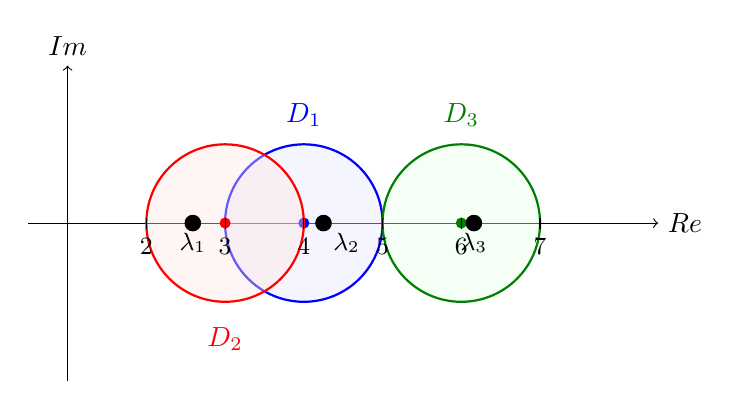
\begin{tikzpicture}[scale=1.0]
    % Axes
    \draw[->] (0.5,0) -- (8.5,0) node[right] {$\operatorname{Re}$};
    \draw[->] (1,-2) -- (1,2) node[above] {$\operatorname{Im}$};

    % Disc D1: center 4, radius 1
    \draw[blue, thick, fill=blue!10, fill opacity=0.4] (4,0) circle (1);
    \node[blue, above] at (4,1.1) {$D_1$};
    \fill[blue] (4,0) circle (2pt);

    % Disc D2: center 3, radius 1
    \draw[red, thick, fill=red!10, fill opacity=0.4] (3,0) circle (1);
    \node[red, below] at (3,-1.2) {$D_2$};
    \fill[red] (3,0) circle (2pt);

    % Disc D3: center 6, radius 1
    \draw[green!50!black, thick, fill=green!10, fill opacity=0.4] (6,0) circle (1);
    \node[green!50!black, above] at (6,1.1) {$D_3$};
    \fill[green!50!black] (6,0) circle (2pt);

    % Eigenvalues (approximate)
    \fill[black] (2.59,0) circle (3pt) node[below] {\small $\lambda_1$};
    \fill[black] (4.25,0) circle (3pt) node[below right] {\small $\lambda_2$};
    \fill[black] (6.16,0) circle (3pt) node[below] {\small $\lambda_3$};

    % Axis labels
    \foreach \x in {2,3,4,5,6,7}
        \draw (\x,0.07) -- (\x,-0.07) node[below] {\small $\x$};
\end{tikzpicture}
\caption{Gerschgorin discs for the matrix $\mathbf{A}$. Black dots indicate the actual eigenvalues.}
\label{fig:gerschgorin}
\end{figure}

%==============================================================================
\section{Power Iteration}
%==============================================================================

\begin{definition}[Power iteration]
\label{def:power-iteration}
\index{power iteration}
The \textbf{power iteration} (or power method) computes the dominant eigenvalue (largest in modulus) and its eigenvector.
\end{definition}

\begin{algorithm}[H]
\caption{Power iteration}
\label{alg:power-iteration}
\KwInput{$\mathbf{A} \in \R^{n \times n}$, initial vector $\mathbf{v}^{(0)}$, tolerance $\varepsilon$, max iterations $k_{\max}$}
\KwOutput{Dominant eigenvalue $\lambda$, eigenvector $\mathbf{v}$}
$\mathbf{v} \gets \mathbf{v}^{(0)} / \|\mathbf{v}^{(0)}\|_2$\;
\For{$k = 1, 2, \ldots, k_{\max}$}{
    $\mathbf{w} \gets \mathbf{A}\,\mathbf{v}$\;
    $\lambda \gets \mathbf{v}^\top \mathbf{w}$ \quad \tcp{Rayleigh quotient}
    $\mathbf{v} \gets \mathbf{w} / \|\mathbf{w}\|_2$\;
    \If{$\|\mathbf{A}\mathbf{v} - \lambda\mathbf{v}\|_2 < \varepsilon$}{
        \Return{$\lambda$, $\mathbf{v}$}\;
    }
}
\Return{$\lambda$, $\mathbf{v}$}\;
\end{algorithm}

\begin{theorem}[Convergence of power iteration]
\label{thm:power-convergence}
\index{power iteration!convergence}
Let $\mathbf{A} \in \R^{n \times n}$ have eigenvalues $|\lambda_1| > |\lambda_2| \geq \cdots \geq |\lambda_n|$ with corresponding eigenvectors $\mathbf{v}_1, \ldots, \mathbf{v}_n$ forming a basis. If $\mathbf{v}^{(0)}$ has a nonzero component in the direction of $\mathbf{v}_1$, then:
\begin{enumerate}
    \item The Rayleigh quotient converges to $\lambda_1$:
    \[
        |\lambda^{(k)} - \lambda_1| = \BigO\!\left(\left|\frac{\lambda_2}{\lambda_1}\right|^{2k}\right).
    \]
    \item The iterates $\mathbf{v}^{(k)}$ converge to $\pm\mathbf{v}_1$ (up to normalization):
    \[
        \|\mathbf{v}^{(k)} - (\pm\mathbf{v}_1)\| = \BigO\!\left(\left|\frac{\lambda_2}{\lambda_1}\right|^k\right).
    \]
\end{enumerate}
The rate of convergence is $r = |\lambda_2/\lambda_1| < 1$.
\end{theorem}

\begin{proof}
Write the initial vector as $\mathbf{v}^{(0)} = \sum_{i=1}^{n} c_i\,\mathbf{v}_i$ with $c_1 \neq 0$. After $k$ iterations (ignoring normalization):
\[
    \mathbf{A}^k\,\mathbf{v}^{(0)} = \sum_{i=1}^{n} c_i\,\lambda_i^k\,\mathbf{v}_i = \lambda_1^k\left[c_1\,\mathbf{v}_1 + \sum_{i=2}^{n} c_i\left(\frac{\lambda_i}{\lambda_1}\right)^k \mathbf{v}_i\right].
\]
Since $|\lambda_i/\lambda_1| < 1$ for $i \geq 2$, the sum converges to $c_1\lambda_1^k\,\mathbf{v}_1$, so the normalized iterate converges to $\pm\mathbf{v}_1$.

For the Rayleigh quotient, $\lambda^{(k)} = (\mathbf{v}^{(k)})^\top\mathbf{A}\,\mathbf{v}^{(k)}$. Since the eigenvector error is $\BigO(r^k)$, the eigenvalue error is $\BigO(r^{2k})$ (the Rayleigh quotient has a quadratic stationary property for symmetric matrices).
\end{proof}

\begin{remark}
The convergence can be very slow when $|\lambda_2/\lambda_1|$ is close to 1. This motivates the use of shifted methods and more sophisticated algorithms.
\end{remark}

%==============================================================================
\section{Inverse Iteration with Shift}
%==============================================================================

\begin{definition}[Inverse iteration with shift]
\label{def:inverse-iteration}
\index{inverse iteration}
To find the eigenvalue closest to a given shift $\sigma$, we apply power iteration to $(\mathbf{A} - \sigma\mathbf{I})^{-1}$, whose dominant eigenvalue is $1/(\lambda_j - \sigma)$ where $\lambda_j$ is the eigenvalue of $\mathbf{A}$ closest to $\sigma$.
\end{definition}

\begin{algorithm}[H]
\caption{Inverse iteration with shift}
\label{alg:inverse-iteration}
\KwInput{$\mathbf{A} \in \R^{n\times n}$, shift $\sigma$, initial $\mathbf{v}^{(0)}$, tolerance $\varepsilon$, $k_{\max}$}
\KwOutput{Eigenvalue $\lambda$ closest to $\sigma$, eigenvector $\mathbf{v}$}
$\mathbf{v} \gets \mathbf{v}^{(0)} / \|\mathbf{v}^{(0)}\|_2$\;
Compute LU factorization of $\mathbf{A} - \sigma\mathbf{I}$\;
\For{$k = 1, 2, \ldots, k_{\max}$}{
    Solve $(\mathbf{A} - \sigma\mathbf{I})\,\mathbf{w} = \mathbf{v}$ \quad \tcp{using LU factors}
    $\lambda \gets \mathbf{v}^\top\mathbf{A}\,\mathbf{v}$ \quad \tcp{Rayleigh quotient}
    $\mathbf{v} \gets \mathbf{w} / \|\mathbf{w}\|_2$\;
    \If{$\|\mathbf{A}\mathbf{v} - \lambda\mathbf{v}\|_2 < \varepsilon$}{
        \Return{$\lambda$, $\mathbf{v}$}\;
    }
}
\Return{$\lambda$, $\mathbf{v}$}\;
\end{algorithm}

\begin{proposition}
Inverse iteration with shift $\sigma$ converges at rate $\left|\frac{\lambda_j - \sigma}{\lambda_k - \sigma}\right|$, where $\lambda_j$ is the nearest eigenvalue to $\sigma$ and $\lambda_k$ is the second nearest. With a good estimate of $\sigma$, convergence can be very fast.
\end{proposition}

\begin{remark}[Rayleigh quotient iteration]
\index{Rayleigh quotient iteration}
If the shift $\sigma$ is updated at each step to the current Rayleigh quotient, we obtain the \textbf{Rayleigh quotient iteration}, which converges cubically for symmetric matrices.
\end{remark}

%==============================================================================
\section{The QR Algorithm}
%==============================================================================

\subsection{Basic QR algorithm}

\begin{definition}[QR algorithm]
\label{def:qr-algorithm}
\index{QR algorithm}
Starting from $\mathbf{A}_0 = \mathbf{A}$, the basic QR algorithm iterates:
\[
    \mathbf{A}_k = \mathbf{Q}_k\,\mathbf{R}_k \qquad (\text{QR factorization}), \qquad
    \mathbf{A}_{k+1} = \mathbf{R}_k\,\mathbf{Q}_k.
\]
\end{definition}

\begin{proposition}[Properties of the QR iteration]
\label{prop:qr-properties}
\begin{enumerate}
    \item All matrices $\mathbf{A}_k$ are similar: $\mathbf{A}_{k+1} = \mathbf{Q}_k^\top\mathbf{A}_k\,\mathbf{Q}_k$.
    \item If $\mathbf{A}$ has eigenvalues $|\lambda_1| > |\lambda_2| > \cdots > |\lambda_n| > 0$, then $\mathbf{A}_k$ converges to an upper triangular matrix with the eigenvalues on the diagonal.
    \item The convergence rate of the sub-diagonal entry $(i+1,i)$ is $\BigO(|\lambda_{i+1}/\lambda_i|^k)$.
\end{enumerate}
\end{proposition}

\subsection{QR algorithm with Hessenberg reduction}

\begin{definition}[Hessenberg form]
\label{def:hessenberg}
\index{Hessenberg form}
A matrix is in \textbf{upper Hessenberg form} if $a_{ij} = 0$ for $i > j+1$:
\[
    \mathbf{H} = \begin{pmatrix}
        h_{11} & h_{12} & h_{13} & \cdots & h_{1n} \\
        h_{21} & h_{22} & h_{23} & \cdots & h_{2n} \\
        0      & h_{32} & h_{33} & \cdots & h_{3n} \\
        \vdots & \ddots & \ddots & \ddots & \vdots \\
        0      & \cdots & 0      & h_{n,n-1} & h_{nn}
    \end{pmatrix}.
\]
\end{definition}

\begin{theorem}[Hessenberg reduction]
\label{thm:hessenberg}
Any matrix $\mathbf{A} \in \R^{n \times n}$ can be reduced to upper Hessenberg form by an orthogonal similarity transformation: $\mathbf{H} = \mathbf{Q}^\top\mathbf{A}\,\mathbf{Q}$, using Householder reflections, in $\BigO(n^3)$ operations.
\end{theorem}

\begin{method}
The practical QR algorithm proceeds in two phases:
\begin{enumerate}
    \item \textbf{Reduction:} Transform $\mathbf{A}$ to Hessenberg form $\mathbf{H}$ (cost: $\BigO(n^3)$, done once).
    \item \textbf{Iteration:} Apply the QR iteration to $\mathbf{H}$, which preserves Hessenberg form. Each QR step on a Hessenberg matrix costs only $\BigO(n^2)$.
\end{enumerate}
For symmetric matrices, Hessenberg form is tridiagonal, and each step costs $\BigO(n)$.
\end{method}

\subsection{QR algorithm with shifts}

\begin{definition}[Shifted QR iteration]
\label{def:shifted-qr}
\index{QR algorithm!shift}
\[
    \mathbf{A}_k - \sigma_k \mathbf{I} = \mathbf{Q}_k\,\mathbf{R}_k, \qquad
    \mathbf{A}_{k+1} = \mathbf{R}_k\,\mathbf{Q}_k + \sigma_k \mathbf{I}.
\]
The shift $\sigma_k$ is chosen to accelerate convergence.
\end{definition}

\begin{definition}[Wilkinson shift]
\label{def:wilkinson-shift}
\index{Wilkinson shift}
The \textbf{Wilkinson shift} is the eigenvalue of the bottom-right $2 \times 2$ submatrix
\[
    \begin{pmatrix} a_{n-1,n-1} & a_{n-1,n} \\ a_{n,n-1} & a_{nn} \end{pmatrix}
\]
that is closer to $a_{nn}$. Explicitly:
\[
    \sigma = a_{nn} + \delta - \operatorname{sign}(\delta)\sqrt{\delta^2 + a_{n,n-1}^2}, \qquad \delta = \frac{a_{n-1,n-1} - a_{nn}}{2}.
\]
\end{definition}

\begin{theorem}
With the Wilkinson shift, the QR algorithm converges cubically for symmetric matrices and at least quadratically in general.
\end{theorem}

\begin{remark}
The complete modern QR algorithm (as implemented in LAPACK) combines:
\begin{itemize}
    \item Hessenberg reduction;
    \item Implicit double shifts (Francis QR step) to handle complex conjugate eigenvalue pairs in real arithmetic;
    \item Deflation when a sub-diagonal element becomes negligible;
    \item Exceptional shifts for difficult cases.
\end{itemize}
The total cost is $\BigO(n^3)$ for all eigenvalues.
\end{remark}

%==============================================================================
\section{Singular Value Decomposition (SVD)}
%==============================================================================

\begin{theorem}[Singular Value Decomposition]
\label{thm:svd}
\index{singular value decomposition}
\index{SVD|see{singular value decomposition}}
Every matrix $\mathbf{A} \in \R^{m \times n}$ (with $m \geq n$) admits a factorization
\[
    \mathbf{A} = \mathbf{U}\,\boldsymbol{\Sigma}\,\mathbf{V}^\top,
\]
where:
\begin{itemize}
    \item $\mathbf{U} \in \R^{m \times m}$ is orthogonal (columns: left singular vectors),
    \item $\mathbf{V} \in \R^{n \times n}$ is orthogonal (columns: right singular vectors),
    \item $\boldsymbol{\Sigma} \in \R^{m \times n}$ is ``diagonal'' with $\sigma_1 \geq \sigma_2 \geq \cdots \geq \sigma_n \geq 0$ (the \textbf{singular values}).
\end{itemize}
\end{theorem}

\begin{proposition}[Properties of the SVD]
\label{prop:svd-properties}
\begin{enumerate}
    \item $\rang(\mathbf{A}) = $ number of nonzero singular values.
    \item $\|\mathbf{A}\|_2 = \sigma_1$, \quad $\|\mathbf{A}\|_F = \sqrt{\sigma_1^2 + \cdots + \sigma_n^2}$.
    \item $\cond_2(\mathbf{A}) = \sigma_1 / \sigma_n$ (when $\mathbf{A}$ is square and invertible).
    \item The singular values of $\mathbf{A}$ are the square roots of the eigenvalues of $\mathbf{A}^\top\mathbf{A}$.
    \item $\mathbf{A} = \sum_{i=1}^{r} \sigma_i\,\mathbf{u}_i\,\mathbf{v}_i^\top$ (outer product form), where $r = \rang(\mathbf{A})$.
\end{enumerate}
\end{proposition}

\begin{theorem}[Eckart--Young theorem]
\label{thm:eckart-young}
\index{Eckart--Young theorem}
The best rank-$k$ approximation to $\mathbf{A}$ (in both the $2$-norm and the Frobenius norm) is
\[
    \mathbf{A}_k = \sum_{i=1}^{k} \sigma_i\,\mathbf{u}_i\,\mathbf{v}_i^\top = \mathbf{U}_k\,\boldsymbol{\Sigma}_k\,\mathbf{V}_k^\top,
\]
where $\mathbf{U}_k$, $\boldsymbol{\Sigma}_k$, $\mathbf{V}_k$ are the truncated SVD. The approximation errors are:
\[
    \|\mathbf{A} - \mathbf{A}_k\|_2 = \sigma_{k+1}, \qquad
    \|\mathbf{A} - \mathbf{A}_k\|_F = \sqrt{\sigma_{k+1}^2 + \cdots + \sigma_n^2}.
\]
\end{theorem}

%==============================================================================
\section{Convergence Study}
%==============================================================================

\begin{example}[Power iteration convergence]
\label{ex:power-convergence}
For the matrix
\[
    \mathbf{A} = \begin{pmatrix} 4 & 1 & 0 \\ 1 & 3 & 1 \\ 0 & 1 & 2 \end{pmatrix},
\]
the eigenvalues are $\lambda_1 \approx 4.732$, $\lambda_2 \approx 3.000$, $\lambda_3 \approx 1.268$. The ratio $r = |\lambda_2/\lambda_1| \approx 0.634$.

\begin{center}
\begin{tabular}{r|cc|cc}
    \toprule
    $k$ & $\lambda^{(k)}$ & $|\lambda^{(k)} - \lambda_1|$ & $|\lambda_2/\lambda_1|^k$ & $|\lambda_2/\lambda_1|^{2k}$ \\
    \midrule
    1  & $4.5000$ & $2.32 \times 10^{-1}$ & $6.34 \times 10^{-1}$ & $4.02 \times 10^{-1}$ \\
    2  & $4.7143$ & $1.77 \times 10^{-2}$ & $4.02 \times 10^{-1}$ & $1.61 \times 10^{-1}$ \\
    3  & $4.7302$ & $1.76 \times 10^{-3}$ & $2.55 \times 10^{-1}$ & $6.48 \times 10^{-2}$ \\
    5  & $4.7321$ & $1.38 \times 10^{-5}$ & $1.02 \times 10^{-1}$ & $1.04 \times 10^{-2}$ \\
    10 & $4.7321$ & $3.32 \times 10^{-11}$ & $1.05 \times 10^{-2}$ & $1.09 \times 10^{-4}$ \\
    \bottomrule
\end{tabular}
\end{center}
The eigenvalue error decreases at rate $\BigO(r^{2k})$ (Rayleigh quotient).
\end{example}

%==============================================================================
\section{Implementations}
%==============================================================================

\begin{codeblock}[title=\textbf{Python --- Eigenvalue algorithms}]
\begin{minted}{python}
import numpy as np
import matplotlib.pyplot as plt

def power_iteration(A, v0=None, tol=1e-12, maxiter=1000):
    """Power iteration for the dominant eigenvalue."""
    n = A.shape[0]
    v = v0 if v0 is not None else np.random.randn(n)
    v = v / np.linalg.norm(v)
    history = []
    for k in range(maxiter):
        w = A @ v
        lam = v @ w  # Rayleigh quotient
        v = w / np.linalg.norm(w)
        history.append(lam)
        if np.linalg.norm(A @ v - lam * v) < tol:
            break
    return lam, v, history

def inverse_iteration(A, sigma, v0=None, tol=1e-12, maxiter=1000):
    """Inverse iteration with shift sigma."""
    n = A.shape[0]
    v = v0 if v0 is not None else np.random.randn(n)
    v = v / np.linalg.norm(v)
    B = A - sigma * np.eye(n)
    lu_piv = None
    try:
        from scipy.linalg import lu_factor, lu_solve
        lu_piv = lu_factor(B)
    except ImportError:
        pass
    history = []
    for k in range(maxiter):
        if lu_piv is not None:
            w = lu_solve(lu_piv, v)
        else:
            w = np.linalg.solve(B, v)
        lam = v @ (A @ v)  # Rayleigh quotient
        v = w / np.linalg.norm(w)
        history.append(lam)
        if np.linalg.norm(A @ v - lam * v) < tol:
            break
    return lam, v, history

def qr_algorithm(A, maxiter=200, tol=1e-12):
    """Basic QR algorithm (without shifts)."""
    n = A.shape[0]
    Ak = A.copy().astype(float)
    for k in range(maxiter):
        Q, R = np.linalg.qr(Ak)
        Ak = R @ Q
        # Check convergence: sub-diagonal elements
        off = np.sum(np.abs(np.tril(Ak, -1)))
        if off < tol:
            break
    return np.diag(Ak), Ak

# Example
A = np.array([[4, 1, 0],
              [1, 3, 1],
              [0, 1, 2]], dtype=float)

print("=== Power iteration ===")
lam, v, hist = power_iteration(A)
print(f"Dominant eigenvalue: {lam:.10f}")
print(f"Eigenvector: {v}")

print("\n=== Inverse iteration (sigma=1.0) ===")
lam2, v2, hist2 = inverse_iteration(A, sigma=1.0)
print(f"Nearest eigenvalue to 1.0: {lam2:.10f}")

print("\n=== QR algorithm ===")
eigenvalues, _ = qr_algorithm(A)
print(f"All eigenvalues: {np.sort(eigenvalues)[::-1]}")

print("\n=== NumPy reference ===")
eigvals = np.linalg.eigvalsh(A)
print(f"numpy.linalg.eigvalsh: {np.sort(eigvals)[::-1]}")

# SVD example
print("\n=== SVD ===")
M = np.array([[3, 2, 2],
              [2, 3, -2]], dtype=float)
U, s, Vt = np.linalg.svd(M)
print(f"Singular values: {s}")
print(f"Rank: {np.sum(s > 1e-10)}")
print(f"||M||_2 = {s[0]:.6f}")
print(f"cond_2(M) = {s[0]/s[-1]:.6f}")

# Low-rank approximation
k = 1
Mk = U[:, :k] @ np.diag(s[:k]) @ Vt[:k, :]
print(f"Best rank-{k} approximation error: {s[k]:.6f}")

# Gerschgorin discs plot
fig, ax = plt.subplots(1, 1, figsize=(8, 4))
for i in range(A.shape[0]):
    center = A[i, i]
    radius = sum(abs(A[i, j]) for j in range(A.shape[1]) if j != i)
    circle = plt.Circle((center, 0), radius, fill=True,
                         alpha=0.2, edgecolor='blue', linewidth=2)
    ax.add_patch(circle)
    ax.plot(center, 0, 'b.', markersize=8)

eigvals_exact = np.linalg.eigvalsh(A)
ax.plot(eigvals_exact, np.zeros_like(eigvals_exact), 'k*',
        markersize=12, label='Eigenvalues')
ax.set_xlim(0, 7)
ax.set_ylim(-2.5, 2.5)
ax.set_aspect('equal')
ax.axhline(y=0, color='gray', linewidth=0.5)
ax.set_xlabel('Re')
ax.set_ylabel('Im')
ax.set_title('Gerschgorin discs')
ax.legend()
plt.tight_layout()
plt.savefig('gerschgorin.pdf')
plt.show()
\end{minted}
\end{codeblock}

\begin{codeblock}[title=\textbf{Julia --- Eigenvalue algorithms}]
\begin{minted}{julia}
using LinearAlgebra, Printf

function power_iteration(A; v0=nothing, tol=1e-12, maxiter=1000)
    n = size(A, 1)
    v = isnothing(v0) ? randn(n) : copy(v0)
    v ./= norm(v)
    lam = 0.0
    for k in 1:maxiter
        w = A * v
        lam = dot(v, w)
        v = w / norm(w)
        if norm(A * v - lam * v) < tol
            @printf("Converged in %d iterations\n", k)
            break
        end
    end
    return lam, v
end

function inverse_iteration(A, sigma; tol=1e-12, maxiter=1000)
    n = size(A, 1)
    v = randn(n)
    v ./= norm(v)
    F = lu(A - sigma * I)
    lam = 0.0
    for k in 1:maxiter
        w = F \ v
        lam = dot(v, A * v)
        v = w / norm(w)
        if norm(A * v - lam * v) < tol
            @printf("Converged in %d iterations\n", k)
            break
        end
    end
    return lam, v
end

# Example
A = [4.0 1.0 0.0;
     1.0 3.0 1.0;
     0.0 1.0 2.0]

println("=== Power iteration ===")
lam, v = power_iteration(A)
@printf("Dominant eigenvalue: %.10f\n", lam)

println("\n=== Inverse iteration (sigma=1.0) ===")
lam2, v2 = inverse_iteration(A, 1.0)
@printf("Nearest eigenvalue to 1.0: %.10f\n", lam2)

println("\n=== Built-in eigvals ===")
println("Eigenvalues: ", eigvals(Symmetric(A)))

println("\n=== SVD ===")
M = [3.0 2.0 2.0; 2.0 3.0 -2.0]
F = svd(M)
println("Singular values: ", F.S)
\end{minted}
\end{codeblock}

%==============================================================================
\section{Exercises}
%==============================================================================

\begin{exercise}[$\star$]
\label{ex:ch10-gerschgorin}
For the matrix
\[
    \mathbf{A} = \begin{pmatrix} 5 & 1 & 1 \\ 0 & 4 & 1 \\ 1 & 0 & -1 \end{pmatrix},
\]
\begin{enumerate}
    \item Determine the three Gerschgorin discs.
    \item Sketch them in the complex plane.
    \item Deduce bounds on the eigenvalues. In particular, show that one eigenvalue is negative.
\end{enumerate}
\end{exercise}

\begin{exercise}[$\star$]
\label{ex:ch10-power-hand}
Apply 3 iterations of power iteration to
\[
    \mathbf{A} = \begin{pmatrix} 2 & 1 \\ 1 & 3 \end{pmatrix}, \qquad \mathbf{v}^{(0)} = \begin{pmatrix} 1 \\ 1 \end{pmatrix}.
\]
Compare the Rayleigh quotient at each step with the exact dominant eigenvalue.
\end{exercise}

\begin{exercise}[$\star\star$]
\label{ex:ch10-inverse-shift}
For the matrix in Exercise~\ref{ex:ch10-power-hand}:
\begin{enumerate}
    \item Apply inverse iteration with shift $\sigma = 1.5$ to find the smallest eigenvalue.
    \item Compare the convergence rate with unshifted power iteration.
\end{enumerate}
\end{exercise}

\begin{exercise}[$\star\star$]
\label{ex:ch10-svd-properties}
Let $\mathbf{A} = \begin{pmatrix} 1 & 2 \\ 3 & 4 \\ 5 & 6 \end{pmatrix}$.
\begin{enumerate}
    \item Compute $\mathbf{A}^\top\mathbf{A}$ and its eigenvalues.
    \item Deduce the singular values of $\mathbf{A}$.
    \item Verify with \texttt{numpy.linalg.svd}.
    \item Compute the best rank-1 approximation and its error.
\end{enumerate}
\end{exercise}

\begin{exercise}[$\star\star$]
\label{ex:ch10-qr-convergence}
Implement the basic QR algorithm and apply it to the matrix
\[
    \mathbf{A} = \begin{pmatrix} 4 & 1 & 0 & 0 \\ 1 & 4 & 1 & 0 \\ 0 & 1 & 4 & 1 \\ 0 & 0 & 1 & 4 \end{pmatrix}.
\]
\begin{enumerate}
    \item Track $\max_{i>j} |a_{ij}^{(k)}|$ (sub-diagonal elements) as a function of iteration $k$.
    \item How many iterations are needed for convergence to $10^{-12}$?
    \item Add the Wilkinson shift and compare.
\end{enumerate}
\end{exercise}

\begin{exercise}[$\star\star\star$]
\label{ex:ch10-image-compression}
\textbf{(Project: Image compression via SVD)}
\begin{enumerate}
    \item Load a grayscale image as a matrix $\mathbf{A} \in \R^{m \times n}$.
    \item Compute its SVD: $\mathbf{A} = \mathbf{U}\boldsymbol{\Sigma}\mathbf{V}^\top$.
    \item Plot the singular values (in log scale). How fast do they decay?
    \item Reconstruct the image using rank-$k$ approximations for $k = 1, 5, 10, 20, 50, 100$.
    \item For each $k$, compute the compression ratio: $\frac{k(m+n+1)}{mn}$.
    \item Plot the relative error $\|\mathbf{A} - \mathbf{A}_k\|_F / \|\mathbf{A}\|_F$ as a function of $k$.
\end{enumerate}
\end{exercise}

\begin{exercise}[$\star\star\star$]
\label{ex:ch10-hessenberg}
Implement Hessenberg reduction using Householder reflections:
\begin{enumerate}
    \item For a general $n \times n$ matrix, compute $\mathbf{H} = \mathbf{Q}^\top\mathbf{A}\mathbf{Q}$.
    \item Verify that $\mathbf{H}$ is upper Hessenberg and $\sigma(\mathbf{H}) = \sigma(\mathbf{A})$.
    \item Implement the QR iteration on the Hessenberg matrix and compare the cost with the basic QR algorithm.
\end{enumerate}
\end{exercise}

%==============================================================================
\section*{Summary of Key Formulas}
%==============================================================================

\begin{keyformulas}
\textbf{Gerschgorin:}
\[
    \sigma(\mathbf{A}) \subset \bigcup_{i=1}^n D_i, \qquad D_i = \{z \in \C : |z - a_{ii}| \leq R_i\}, \quad R_i = \sum_{j \neq i} |a_{ij}|
\]

\textbf{Power iteration:} converges to $\lambda_1$ at rate $|\lambda_2/\lambda_1|^k$ (eigenvector) or $|\lambda_2/\lambda_1|^{2k}$ (Rayleigh quotient).

\textbf{Inverse iteration with shift $\sigma$:} converges to the eigenvalue nearest $\sigma$, rate $\left|\frac{\lambda_j - \sigma}{\lambda_k - \sigma}\right|^k$.

\textbf{QR algorithm:}
\[
    \mathbf{A}_k = \mathbf{Q}_k\mathbf{R}_k, \quad \mathbf{A}_{k+1} = \mathbf{R}_k\mathbf{Q}_k \quad \to \quad \text{upper triangular (eigenvalues on diagonal)}
\]

\textbf{Wilkinson shift:} $\sigma = a_{nn} + \delta - \operatorname{sign}(\delta)\sqrt{\delta^2 + a_{n,n-1}^2}$, $\delta = (a_{n-1,n-1} - a_{nn})/2$.

\textbf{SVD:} $\mathbf{A} = \mathbf{U}\boldsymbol{\Sigma}\mathbf{V}^\top$, \quad $\|\mathbf{A}\|_2 = \sigma_1$, \quad $\cond_2(\mathbf{A}) = \sigma_1/\sigma_n$.

\textbf{Eckart--Young:} Best rank-$k$ approximation is truncated SVD, error $= \sigma_{k+1}$ (2-norm).
\end{keyformulas}
